\chapter{Einleitung (Exposé)}
\label{ch:einleitung}

\section*{Problemstellung und Relevanz}
\label{sec:problemstellung}
Die deutsche Bau-- und Infrastrukturbranche steht vor immensen Herausforderungen, die  eine grundlegende Steigerung der Effizienz und Umsetzungsgeschwindigkeit erfordern.  Ein signifikantes Wohnungsbaudefizit, das je nach Studie auf über 550.000 fehlende  Wohnungen beziffert wird, verlangt nach einer drastischen Beschleunigung des Neubaus\autocite[]{}. Gleichzeitig stellt die  Bundesregierung über ein neues Sondervermögen für Infrastruktur und Klimaschutz bis  2029 mehr als 100 Milliarden Euro an Mitteln jeweils für den Bahn- und Wohnungsbau  bereit\autocite[]{brinkmeier2025}. Die Umsetzung der bereitgestellten Mittel in den dringend  benötigten Projekten droht jedoch an strukturellen Problemen wie dem eklatanten  Fachkräftemangel, anhaltenden Kapazitätsengpässen in der Bauwirtschaft und  langwierigen Genehmigungsverfahren zu scheitern\autocite[]{hdb2025}.

\begin{figure}[htbp]
    \centering
    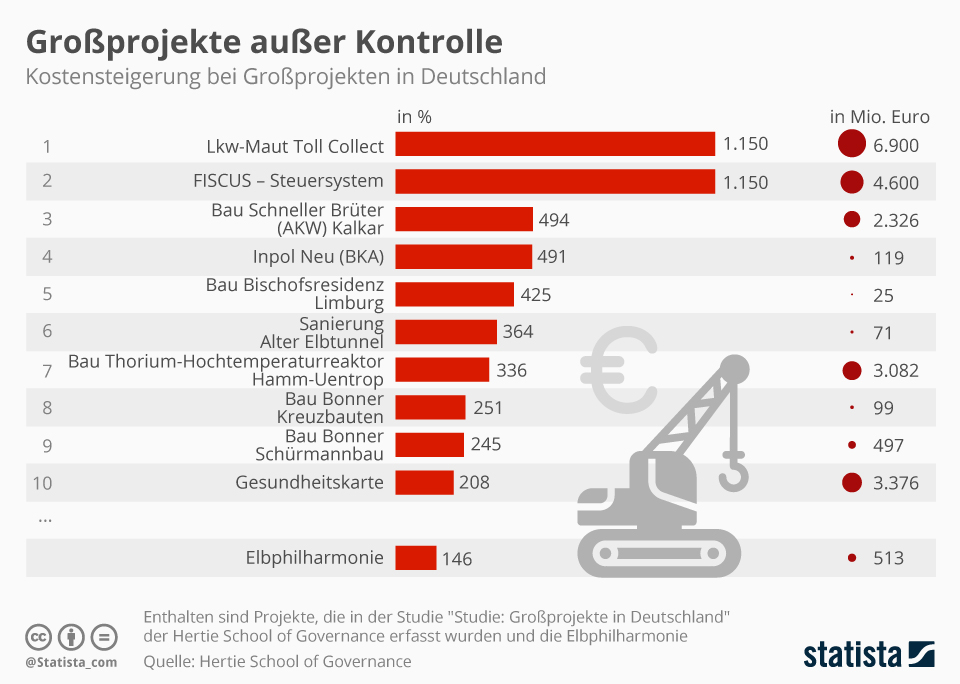
\includegraphics[width=0.9\textwidth]{kostensteigerung-grossprojekte-deutschland}
    \caption{Kostensteigerungen bei deutschen Großprojekten \cite{statista2024grossprojekte}}
    \label{fig:kostensteigerung-grossprojekte}
\end{figure}
\clearpage
Zusätzlich steht diese Bedarfslage einer traditionell fragmentierten und sequentiell  organisierten Projektabwicklung gegenüber. Die etablierte Projektkultur, die stärker auf  vertragliche Abgrenzung als auf Zusammenarbeit ausgerichtet ist, begünstigt strukturelle  Ineffizienzen sowie Kosten-- und Terminüberschreitungen, die bei öffentlichen  Großprojekten im Durchschnitt bei über 40\% liegen\autocite[]{korn2019}. Vor dem  Hintergrund der aktuellen Herausforderungen erscheinen diese Eigenschaften  zunehmend problematisch.

Ein vielversprechender Lösungsansatz, welcher sich international bereits etabliert hat,  bieten integrierte Projektabwicklungsmodelle wie das Project Alliancing oder die  Integrierte Projektabwicklung (IPA). Bei diesen Arten der Projektabwicklung liegt der  Fokus auf einem kollaborativen, gemeinschaftlichen Ansatz, bei dem die wesentlichen  Akteure frühzeitig in einem Mehrparteienvertrag gebunden werden, um Risiken und  Chancen gemeinsam zu managen und das Projekt auf den Gesamterfolg auszurichten.  Dieser Ansatz hat sich international als äußerst erfolgreich bei der Realisierung  komplexer Vorhaben bewährt\autocite[]{cook2014}.

In den letzten Jahren hat das IPA--Thema auch in Deutschland stark an Fahrt aufgenommen und findet derzeit in mehr und mehr Pilotprojekten Anwendung. Das IPA--Zentrum identifizierte in seinem Jahresbericht von 2024 insgesamt 25 abgeschlossene oder laufende IPA--Projekte und weitere, bei denen eine aktive Entscheidung für IPA bereits gefallen ist (vgl. Haghsheno et al 2024). Ein zentraler Prozessbaustein zur Kosten-- und Wertsteuerung innerhalb dieser Modelle ist das Target Value Design (TVD)\autocite[]{Testkey}. Während zu den übergeordneten IPA--Rahmenbedingungen bereits Forschung im deutschen Kontext existiert\autocite[]{haghsheno2024}, fehlt eine systematische, prozessorientierte  Aufbereitung für die Anwendung von TVD (siehe Kapitel 3). Hier setzt die vorliegende  Arbeit an, um diese Lücke zu schließen und aufzuzeigen, wie TVD als Methode zur Bewältigung der anstehenden Bauaufgaben beitragen kann.

\section*{Zielsetzung und Forschungsfrage}
\label{sec:zielsetzung}

\subsection*{Hauptziel und zentrale Forschungsfrage}
Das Hauptziel dieser Arbeit besteht in der systematischen Analyse und Aufbereitung des Target Value Design (TVD) als zentraler Bestandteil moderner, integrierter Projektabwicklungsmodelle im Bauwesen wie der Integrierten Projektabwicklung (IPA). Dabei sollen, anhand einer systematischen Literaturrecherche, wesentliche Prozessbausteine des TVD identifiziert und beschrieben werden, um sie anschließend zu einem idealtypischen Gesamtprozess zusammenzusetzen. Die tiefgehende Aufbereitung und Darstellung sollen im Anschluss eine optimale Gegenüberstellung mit den Abläufen der konventionellen Projektabwicklung in Deutschland ermöglichen. Dieser Vergleich konzentriert sich insbesondere auf die Rahmenbedingungen in der deutschen Baupraxis, die von den einschlägigen Regelwerken wie HOAI und AHO geschaffen werden, und dient vor allem der Identifizierung von Anpassungsbedarfen. Letztere sollen schlussendlich in der Ableitung eines Transferleitfadens münden, der die Anwendung von TVD im Kontext der Bauprojektabwicklung in Deutschland verbessert.

Daraus leitet sich die folgende zentrale Forschungsfrage ab:

\enquote{Wie lässt sich der Target Value Design-Prozess strukturiert in Einzelschritte zerlegen, nachvollziehbar darstellen und für die Anwendung in der deutschen Baupraxis übersetzen, um den strukturellen Defiziten der traditionellen Projektabwicklung entgegenzuwirken?}

\subsection*{Exploratives Nebenziel}
Ergänzend zum Hauptziel soll diese Arbeit einen explorativen Ausblick auf eine weitere Forschungslücke, die mögliche Übertragbarkeit von TVD im Hochbau auf Infrastrukturprojekte \autocite [S.45]{ballard2025}, gewähren. Ziel ist es aufzuzeigen, welche spezifischen Charakteristika diese Bauprojektarten (z.\,B. Linienbaustellen) aufweisen und welche der zuvor herausgearbeiteten Bausteine des TVD hier potenziell anwendbar wären bzw. einer Anpassung bedürfen.

\subsection*{Hypothese und erwartete Erkenntnisse}
Die zentrale Hypothese dieser Arbeit lautet, dass eine direkte Übertragung des TVD-Prozesses auf die deutsche Baupraxis aufgrund der strukturellen, rechtlichen und kulturellen Rahmenbedingungen nicht zielführend ist. Vielmehr wird angenommen, dass eine erfolgreiche Implementierung von Target Value Design über die bloße Einführung einer Methode hinausgeht und spezifische Anpassungen erfordert, um den Gegebenheiten in Deutschland gerecht zu werden.
Als Ergebnis dieser Arbeit soll ein Transferleitfaden für die Anwendung von Target Value Design in Deutschland entstehen. Dieser Leitfaden soll sowohl den aufbereiteten Prozess darstellen als auch Inkompatibilitäten aufzeigen und konkrete Handlungsempfehlungen für letztere bieten, um eine effiziente Projektabwicklung mit Target Value Design zu ermöglichen.

\section*{Methodischer Ansatz}
\label{sec:methodischer-ansatz}

Die Arbeit verfolgt einen literaturbasierten, konzeptionell-analytischen Forschungsansatz, der sich in drei aufeinander aufbauende Schritte gliedert:

\begin{enumerate}
    \item \textbf{Systematische Literaturrecherche und -analyse:} Zunächst werden die theoretischen Grundlagen durch eine systematische Literaturrecherche erarbeitet. Dabei werden einschlägige wissenschaftliche Datenbanken (z.\,B. Scopus, Web of Science) sowie relevante Publikationen von Fachinstitutionen (z.\,B. LCI, GLCI, IPA-Zentrum) ausgewertet. Die Recherche wird durch gezielte Suchstrategien (Keyword Kombinationen) und Auswahlkriterien (z.\,B. Aktualität, Relevanz) strukturiert, um internationale Standardwerke zu TVD und IPA sowie Fachliteratur zu den spezifischen Rahmenbedingungen der deutschen Baupraxis zu identifizieren und zu analysieren.
    
    \item \textbf{Prozessbeschreibung und Modellierung:} Auf Basis der analysierten Literatur wird ein idealtypisches Prozessmodell des TVD konstruiert. Dieses Modell zerlegt den Gesamtprozess in seine wesentlichen Phasen, Rollen, Entscheidungspunkte und Abhängigkeiten und visualisiert deren Zusammenspiel.
    
    \item \textbf{Kontextanalyse und Ableitung des Transferleitfadens:} Das idealtypische TVD-Modell wird anschließend den strukturellen, technischen, rechtlichen und kulturellen Gegebenheiten der deutschen Baupraxis im Hochbau gegenübergestellt. Aus dieser Gegenüberstellung werden Reibungspunkte und Anpassungsbedarfe identifiziert. Die Ergebnisse münden in der Entwicklung eines konzeptionellen Transferleitfadens, der konkrete Handlungsempfehlungen für die Anwendung von TVD in Deutschland formuliert.
\end{enumerate}

Für das explorative Nebenziel der Übertragbarkeit von TVD auf Infrastrukturprojekte werden die aus dem Hochbau gewonnenen Erkenntnisse auf die spezifischen Charakteristika dieser Projektart angewandt, um erste Hypothesen für notwendige Adaptionen aufzuzeigen.

\section*{Aufbau der Arbeit}
\label{sec:aufbau}
